\chapter{Análisis Formal de Conceptos.}\label{cap:capitulo2}

En este capítulo se formalizan algunas nociones sobre {\bf Análisis Formal de Conceptos} (AFC), que serán necesarias para comprender algunas de las técnicas que se usan en el trasfondo de este trabajo. Las definiciones básicas en AFC son las de Contexto Formal y Concepto Formal. El adjetivo \emph{formal} se usa simplemente para indicar que existe un trasfondo matemático en ambas definiciones, y por tanto, su significado difiere de aquellos que tienen en el lenguaje natural.

A lo largo de todo el capítulo, se incluirá un ejemplo que ilustre todas las definiciones que se van incluyendo. Se ha escogido un ejemplo de pequeño tamaño, para facilitarle al lector la lectura y comprensión del proceso; así como la representación de los resultados que se van obteniendo. Sin embargo, estas técnicas que var a ser definidas en este capítulo, serán usadas en el desarrollo de este trabajo con muestras de un tamaño mucho mayor; y por tanto, los resultados serán igualmente de mayor tamaño, por lo que será mucho más difícil representarlos gráficamente.

Se recomienda consultar \cite{afc} como recurso bibliográfico, en el que se formaliza las definiciones de \emph{conjunto}, \emph{conjunto ordenado} o \emph{retículos completos}, que utilizaremos a lo largo de todo el capítulo. Además, se incluyen las demostraciones de todos los teoremas aquí presentados.

\section{Contextos Formales.}

\begin{defi}
	Un {\bf Contexto Formal} $\K := (G, M, I)$ está compuesto por dos conjuntos $G$ y $M$ y una relación $I$ entre $G$ y $M$ ($I \subseteq \{G \times{M}\}$). Los elementos de $G$ son los {\bf objetos} (formales) y los elementos de $M$ son los {\bf atributos} (formales) del Contexto. La relación entre un objeto $g\in{G}$ y un atributo $m\in{M}$, se expresa como $(g,m)\in{I}$ (o $gIm$), y se lee como ``el objeto $g$ tiene el atributo $m$".
\end{defi}

En el siguiente ejemplo, se ilustra un pequeño contexto sobre peces (objetos) y los hábitats en los que viven (atributos):

\begin{itemize}
	\item Un conjunto de Objetos $G$, que son los peces que forman parte de este contexto: carpa, escatófagus, sargo, dorada y anguila.
	\item Un conjunto de Atributos $M$, que son las posibles características de los objetos anteriores, y que en este ejemplo expresan los posibles hábitats de los peces (que no tienen porqué ser exclusivos): fluvial, litoral y océano.
	\item Una relación $I$, entre $G$ y $M$, expresada en la tabla~\ref{fig:contexto}.
\end{itemize}

\begin{figure}[h]

\centering
{ 
\begin{tabular}{|l|c|c|c|}
\hline
& Océano & Litoral & Fluvial \\
\hline
Sargo &  X  &  X  &    \\ \hline
Dorada &  X  &  X  &    \\ \hline
Carpa &    &    &  X  \\ \hline
Anguila &  X  &  X  &  X  \\ \hline
Escatófagus &    &  X  &  X  \\ \hline
\end{tabular}
}
\caption{Ejemplo de Contexto Formal
\label{fig:contexto}
}

\end{figure}

Como se ve en el ejemplo anterior, un contexto puede ser expresado fácilmente en una tabla de doble entrada, dónde las filas se corresponden con los objetos, y las columnas con los atributos. La relación entre ambos se expresa marcando las casillas correspondientes, de forma que si la casilla de la fila $g$ y columna $m$ está marcada, significa que el objeto $g$ tiene el atributo $m$; es decir que $(g,m)\in{I}$, (o $gIm$). En caso contrario, la casilla quedará sin marcar.

De esta forma, se ve como un objeto puede tener múltiples atributos, y un atributo puede pertenecer a varios objetos.

Denotaremos $\{...\}_{\cal X}$ a un subconjunto de elementos del conjunto ${\cal X}$; es decir que $\{...\}_G$ es un subconjunto de objetos, y $\{...\}_M$ es un subconjunto de atributos.



\section{Intención y Extensión.}

Se definen los conjuntos $A'$ y $B'$, de Intención y Extensión de un Contexto ${\cal K} := (G,M,I)$, como:

\begin{defi}
Para un contexto ${\cal K} := (G,M,I)$ y un conjunto $A\in{G}$ de objetos, se define la {\bf Intención} como el conjunto $A'$; que es precisamente el conjunto de atributos comunes a los objetos de $A$:
\begin{center}
$A' := \{m\in{M}|\ gIm\ \forall{g\in{A}}\}$
\end{center}
\end{defi}

\begin{defi}
Para un contexto ${\cal K} := (G,M,I)$ y un conjunto $B\in{M}$ de atributos, se define la {\bf Extensión} como el conjunto $B'$; que es precisamente el conjunto de objetos comunes a los atributos de $B$: 
\begin{center}
$B' := \{g\in{G}|\ gIm\ \forall{m\in{B}}\}$
\end{center}
\end{defi}

Veamos algunos ejemplos de estas operaciones sobre nuestro contexto ejemplo (figura~\ref{fig:contexto}) para ilustrar estas operaciones:
\begin{itemize}
	\item (1): $\{\ fluvial,\ oc\acute{e}ano\ \}'_M\ =\ \{\ anguila\ \}_G$
	\item (2): $\{\ carpa,\ sargo\ \}'_G\ =\ \emptyset_M$
	\item (3): $\{\ escat\acute{o}fagus,\ sargo\ \}'_G\ =\ \{\ litoral\ \}_M$
\end{itemize}

El ejemplo (1) es un ejemplo de extensión de atributos, mientras que los ejemplos (2) y (3) son ejemplos de intención de objetos.







\section{Conceptos Formales.}

\begin{defi}
Un {\bf Concepto Formal} de un Contexto ${\cal K}:=(G,M,I)$ es un par $(A,B)$ con $A \subseteq G$, $B \subseteq M$, tal que $A' = B$ y $B' = A$, dónde $A'$ y $B'$ son respectivamente la extensión y la intención del concepto $(A,B)$.
\end{defi}

Veamos algunos ejemplos para identificar qué es y qué no es un concepto sobre el contexto de nuestro ejemplo (figura~\ref{fig:contexto}):
\begin{itemize}
	\item (1): $ (\{sargo,\ dorada,\ anguila\}, \{litoral,\ oc\acute{e}ano\}) $ es un concepto; porque:
	\begin{itemize}
		\item $\{sargo,\ dorada,\ anguila\}'\ =\ \{litoral,\ oc\acute{e}ano\}$
		\item $\{litoral,\ oc\acute{e}ano\}'\ =\ \{sargo,\ dorada,\ anguila\}$
	\end{itemize}
	\item (2): $ (\emptyset_G,\ \emptyset_M) $ no es un concepto; porque:
	\begin{itemize}
		\item $ \emptyset_G'\ =\ M\ \neq\ \emptyset_M $
	\end{itemize}
	\item (3): $ (G,\ \emptyset_M) $ es un concepto; porque:
	\begin{itemize}
		\item No existe ningún atributo común a todos los objetos; es decir:
		\item $ G'\ =\ \emptyset_M $
		\item $ \emptyset_M'\ =\ G $
	\end{itemize}
	\item (4): $ (\emptyset_G,\ M) $ no es un concepto pues:
	\begin{itemize}
		\item Aunque $ \emptyset_G'\ = M $,
		\item se tiene $ M'\ =\ \{anguila\}\ \neq\ \emptyset_G $
	\end{itemize}
\end{itemize}

Los ejemplos (1) y (3) son conceptos porque la extensión del subconjunto de atributos es precisamente el subconjunto de objetos, y la intención del subconjunto de objetos es precisamente el subconjunto de atributos. Los ejemplos (2) y (4) no son conceptos porque no se cumplen alguna de estas dos condiciones.

\begin{defi}
Si $(A_1, B_1)$ y $(A_2, B_2)$ son conceptos de un contexto, $(A_1, B_1)$ es un {\bf subconcepto} de $(A_2, B_2)$ si $A_1 \subseteq A_2$ (o equivalentemente si $B_2 \subseteq B_1$). En este caso, $(A_2, B_2)$ es un {\bf superconcepto} de $(A_1, B_1)$, y se escribe como $(A_1, B_1) \leq (A_2, B_2)$. La relación $\leq$ se llama {\bf orden de jerarquía} (o simplemente {\bf orden}) de los conceptos.
\end{defi}



\section{Retículos de Conceptos.}

En la sección anterior se ha visto que los conceptos pueden ser ordenados jerárquicamente. Esto permite crear un conjunto ordenado de todos ellos.

\begin{defi}
El conjunto ordenado de todos los conceptos de un contexto ${\cal K}:=(G,M,I)$, se denota como ${\cal B}(G,M,I)$, y se llama {\bf retículo de conceptos}.
\end{defi}

En el ejemplo que estamos ilustrando, se obtienen los siguientes conceptos:
\begin{itemize}
	\item $C_0 := (\{anguila, carpa, dorada, escat\acute{o}fagus, sargo\}_G, \emptyset_M)$
	\item $C_1 := (\{anguila, carpa, escat\acute{o}fagus\}_G, \{fluvial\}_M)$
	\item $C_2 := (\{anguila, dorada, escat\acute{o}fagus, sargo\}_G, \{litoral\}_M)$
	\item $C_3 := (\{anguila, escat\acute{o}fagus\}_G, \{litoral, fluvial\}_M)$
	\item $C_4 := (\{anguila, dorada, sargo\}_G, \{litoral, oc\acute{e}ano\}_M)$
	\item $C_5 := (\{anguila\}_G, \{litoral, fluvial, oc\acute{e}ano\}_M)$
\end{itemize}

Y se obtienen las siguientes relaciones de orden entre los conceptos:
\begin{itemize}
  \begin{minipage}[t]{0.3\linewidth} \centering
	\item $C_0 \geq C_1$
	\item $C_0 \geq C_2$
	\item $C_1 \geq C_3$
	\item $C_2 \geq C_3$
  \end{minipage}
   \hspace{0.5cm}
   \begin{minipage}[t]{0.3\linewidth} \centering
	\item $C_2 \geq C_4$
	\item $C_3 \geq C_5$
	\item $C_4 \geq C_5$
   \end{minipage}
\end{itemize}

El retículo de conceptos se puede representar fácilmente en una estructura de grafo, de forma que cada nodo se corresponderá con cada uno de los conceptos que se obtienen del contexto que se representa. Por tanto, habrá tantos nodos como número de conceptos. La relación de orden se expresará en la dirección vertical del grafo, de forma que si un concepto es subconcepto de otro, el superconcepto estará posicionado más arriba que el subconcepto. Por último, y para evitar repeticiones innecesarias en la escritura de los objetos y los atributos, sólo se expresarán una única vez. Los objetos se expresarán en el nodo más bajo posible, de forma que todos los nodos superiores a éste, también contienen a dicho objeto. Los atributos se expresarán en el nodo más alto posible, de forma que todos los nodos inferiores a éste, también contienen a dicho atributo. En la figura~\ref{fig:reticulo}, vemos el grafo obtenido de este retículo de conceptos.

\begin{figure}[t]
\centering
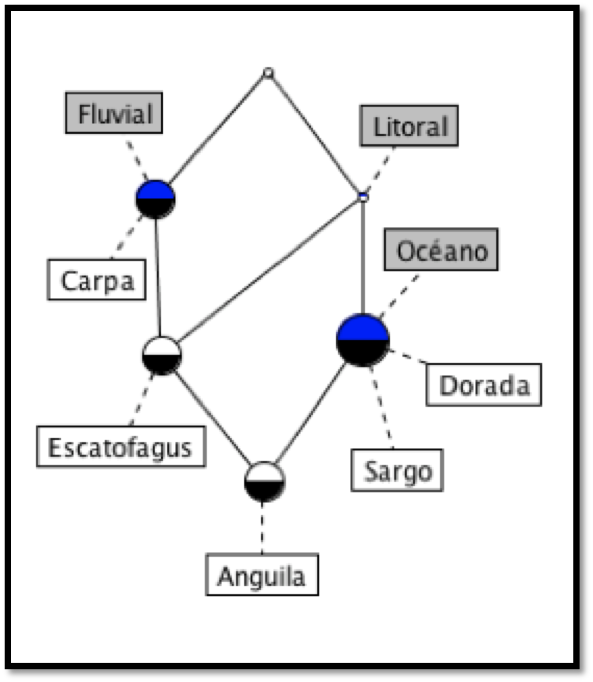
\includegraphics[scale=0.75]{img/2/reticulo}
\caption{Retículo de Conceptos
\label{fig:reticulo}}
\end{figure}



\section{Bases Stem.}

\begin{defi}
Para un contexto ${\cal K}:=(G,M,I)$, Una {\bf implicación} entre atributos es una expresión de la forma $Y_1 \rightarrow{Y_2}$, dónde $Y_1, Y_2 \subseteq M$; es decir, son subconjuntos de atributos.
\end{defi}

El objetivo es obtener un conjunto de relaciones entre los atributos, para que, usando operaciones lógicas, se pueda trabajar con el contexto dado.

A continuación se definen una serie de características sobre las implicaciones. Sea ${\cal L}$ un conjunto de implicaciones; se tiene:
\begin{enumerate}
	\item ${\cal L} \ \models Y \rightarrow{Z}$ ($Y \rightarrow{Z}$ es {\bf consecuencia} de ${\cal L}$) si para todo $T \subseteq M$, si $T$ respeta ${\cal L}$ entonces $T$ respeta $Y \rightarrow{Z}$.
	\item ${\cal L}$ es {\bf cerrada} si contiene a toda implicación $Y \rightarrow{Z}$ que es consecuencia de ${\cal L}$.
	\item ${\cal L}$ es {\bf completo} si toda implicación válida en $(G,M,I)$ es consecuencia de ${\cal L}$:
	\begin{center}
		$(G,M,I) \models Y \rightarrow{Z}\ \ \Longrightarrow{\ \  {\cal L} \ \models Y \rightarrow{Z} }$
	\end{center}
	\item ${\cal L}$ es {\bf no redundante} si ninguna implicación de ${\cal L}$ es consecuencia del resto:
	\begin{center}
		$Y \rightarrow{Z} \in{{\cal L}}\ \ \Longrightarrow{\ \  {\cal L} \backslash \{ Y \rightarrow{Z}\} \not\models Y \rightarrow{Z} }$
	\end{center}
\end{enumerate}

\begin{defi}
	Se define como {\bf Base Stem} al conjunto {\bf completo} e {\bf irredundante} de implicaciones de un contexto ${\cal K}:=(G,M,I)$.
\end{defi}

El problema se reduce, pues, a obtener una Base Stem para un contexto dado. Para ello, se hará uso del cálculo implicacional basado en las Reglas de Amstrong:

\begin{center}
\begin{minipage}[t]{0.3\linewidth} \centering
	$R_1: \frac{}{X\rightarrow{X}}$
\end{minipage}
%\hspace{0.5cm}
\begin{minipage}[t]{0.3\linewidth} \centering
	$R_2: \frac{X\rightarrow{Y}}{X \cup Z \rightarrow{Y}}$
\end{minipage}
%\hspace{0.5cm}
\begin{minipage}[t]{0.3\linewidth} \centering
	$R_3: \frac{X\rightarrow{Y}, Y \cup Z \rightarrow{W}}{X \cup Z \rightarrow{W}}$
\end{minipage}
\end{center}

Con este conjunto de reglas, se puede obtener el siguiente cálculo lógico:

\begin{center}
	${\cal L} \vdash L \Longleftrightarrow{L}$ se prueba mediante las reglas de Amstrong a partir de ${\cal L}$.
\end{center}

\begin{teo}
	Si ${\cal L}$ es un conjunto Stem para un contexto formal ${\cal K}$, entonces ${\cal L}$ proporciona una teoría implicacionalmente completa para ese modelo; es decir:
	\begin{center}
	$ {\cal L} \vdash L \Longrightarrow{ {\cal K} \models L }$
	\end{center}
\end{teo}

\begin{defi}
	$P \subseteq M$ es una {\bf pseudointención} de un contexto ${\cal K}:=(G,M,I)$ si se verifica que:
	\begin{itemize}
		\item $P \neq P''$
		\item Para toda pseudointención $Q \subset P$, se verifica que $Q'' \subseteq P$.
	\end{itemize}
\end{defi}

\begin{teo}
	El conjunto $\{P \rightarrow {P''} | P \mbox{ es pseudointención}\}$ es una Base Stem del Contexto. \\
	En la práctica, únicamente se toman las implicaciones $P \rightarrow {(P''-P)}$, ya que $P \rightarrow {P}$ siempre es válido.
\end{teo}

A cada pseudointención podemos añadirle un atributo de {\bf soporte}, que indica el número de objetos que cumplen esta implicación. Este soporte será un entero mayor o igual a cero.

Veamos en nuestro ejemplo, la traza del algoritmo seguido para calcular las distintas pseudointenciones del contexto. Dado que la definición de pseudointención es recursiva, iniciaremos con el conjunto vacío, e iremos recorriendo los subconjuntos de menor a mayor tamaño. De esta forma, las pseudointenciones calculadas previamente nos pueden ayudar a descartar otras pseudointenciones en el proceso. Por mejorar la visibilidad, únicamente se expresarán las iniciales de los atributos y de los objetos.

\begin{itemize}
	\item $\emptyset_M = G = \emptyset_M$; por tanto, NO.
	\item $\{f\}'' = \{c,e,a\}' = \{f\}$; por tanto, NO.
	\item $\{l\}'' = \{e,s,d,a\}' = \{l\}$; por tanto, NO.
	\item $\{o\}'' = \{s,d,a\}' = \{l,o\}$; por tanto, SÍ.
	\item $\{f,l\}'' = \{e,a\}' = \{f,l\}$; por tanto, NO.
	\item $\{f,o\}'' = \{a\}' = \{f,l,o\}$; sin embargo se tiene que $\{o\}\subset\{f,o\}$, \\ y $\{o\}'' = \{l,o\} \not\subseteq \{f,o\}$; por tanto NO.
	\item $\{l,o\}'' = \{s,d,a\}' = \{l,o\}$; por tanto NO.
	\item $\{f,l,o\}'' = \{a\}' = \{f,l,o\}$; por tanto, NO.
\end{itemize}

Por tanto, la Base Stem obtenida (simplificando las implicaciones) en el ejemplo que hemos seguido a lo largo de todo el capítulo, es:
\begin{itemize}
	\item $(\{oceanico\} \rightarrow {\{litoral\}})$, con soporte 3 (puesto que 3 objetos la cumplen).
\end{itemize}


